\PassOptionsToPackage{pdfpagelabels=false}{hyperref}
\documentclass[fleqn,usenatbib,usedcolumn]{mnras}
%==============================================================================%
\usepackage[british]{babel}             % British English hyphenation
\usepackage{txfonts}                  % Good fonts
% Use vector fonts, so it zooms properly in on-screen viewing software
% Don't change these lines unless you know what you are doing
%\usepackage[T1]{fontenc}
%\usepackage{ae,aecompl}
%%%%% AUTHORS - PLACE YOUR OWN PACKAGES HERE %%%%%
\usepackage{graphicx}	% Including figure files
\usepackage{hyperref} % hyperlinks
\usepackage{natbib}
\usepackage{aastexmacros}
\usepackage{tikz}
\usepackage[caption=false]{subfig}
\usepackage[mediumspace,mediumqspace,Grey,squaren]{SIunits}
%%%%%%%%%%%%%%%%%%%%%%%%%%%%%%%%%%%%%%%%%%%%%%%%%%

%%%%% AUTHORS - PLACE YOUR OWN COMMANDS HERE %%%%%
\usetikzlibrary{shapes,arrows,calc,positioning}

\renewcommand{\vec}[1]{\mathbf{#1}}
% \newcommand{\text}{\mathrm}
\newcommand{\jansky}{\text{Jy}}
\newcommand{\cheng}[1]{ {\color{teal}[{\bf Cheng TODO:~{#1}}]} }
\newcommand{\matthew}[2]{ {\color{white!20!violet}[{\bf TODO(#1):~{#2}}]} }
\newcommand{\todo}[1]{ {\color{red}[{\bf TODO:~{#1}}]} }


\newcommand{\underset}[2]{\mathop{#2}\limits_{#1}}

\let\subsectionautorefname\sectionautorefname
\let\subsubsectionautorefname\sectionautorefname

%%%%%%%%%%%%%%%%%%%%%%%%%%%%%%%%%%%%%%%%%%%%%%%%%%

%%%%%%%%%%%%%%%%%%% TITLE PAGE %%%%%%%%%%%%%%%%%%%

\title[Supplement: ML for radio X-id]{Supplement to Radio Galaxy Zoo: Machine learning methods for radio source host galaxy cross-identification}

\author[Alger et al.]{
  M.~J.~Alger$^{1}$,
  J.~K.~Banfield$^{2, 1}$,
  C.~S.~Ong$^{3, 4}$,
  O.~I.~Wong$^{5, 2}$,
  L.~Rudnick$^{6}$,
  R.~P.~Norris$^{7, 8}$, others
\\
% List of institutions
$^{1}$Research School of Astronomy and Astrophysics, The Australian National University, Canberra, ACT 2611, Australia\\
$^{2}$ARC Centre of Excellence for All-Sky Astrophysics (CAASTRO)\\
$^{3}$Data61, CSIRO, Canberra, ACT 2601, Australia\\
$^{4}$Research School of Computer Science, The Australian National University, Canberra, ACT 2601, Australia\\
$^{5}$International Centre for Radio Astronomy Research-M468, The University of Western Australia, 35 Stirling Hwy, Crawley, WA 6009, Australia\\
$^{6}$Minnesota Institute for Astrophysics, University of Minnesota, 116 Church St. SE, Minneapolis, MN 55455\\
$^{7}$Western Sydney University, Locked Bag 1797, Penrith South, NSW 1797, Australia\\
$^{8}$CSIRO Astronomy \& Space Science, PO Box 76, Epping, NSW 1710, Australia
}

% These dates will be filled out by the publisher
\date{Accepted XXX. Received XXX}

% Enter the current year, for the copyright statements etc.
\pubyear{2017}

% Don't change these lines
\begin{document}
\label{firstpage}
\pagerange{\pageref{firstpage}--\pageref{lastpage}}
\maketitle


  \section{Classifiers}\label{sec:classifiers}

    We use three different classifiers as our binary classification model:
    logistic regression, convolutional neural networks, and random forests.

    \subsection{Logistic Regression}
    \label{sec:logistic-regression}
      Logistic regression is a binary classification model. It is linear in the
      feature space and outputs the probability that the input has a positive
      label. The model is \citep{bishop06ml}:

      \begin{equation}
          f(\vec x) = \sigma(\vec w \cdot \vec x + b) \,\,\,\,,
      \end{equation}
      where $\vec w \in \mathbb{R}^D$ is a weight vector,
      $b \in \mathbb{R}$ is a bias term, $\vec x \in \mathbb{R}^D$ is the
      feature representation of a candidate host, and $\sigma$ is the
      logistic sigmoid function: \begin{equation}
          \sigma(a) = (1 + \mathrm{exp}(-a))^{-1}\,\,\,\,.
      \end{equation}%
      The logistic regression model is fully differentiable, and the weight
      vector $\vec w$ can therefore be learned using gradient methods.

    \subsection{Convolutional neural networks}
    \label{sec:convolutional-neural-networks}

      Convolutional neural networks (CNN) are a biologically-inspired
      prediction model for prediction with image inputs. The input image is
      convolved with a number of filters to produce output images called
      feature maps. These feature maps can then be convolved again with other
      filters on subsequent layers, producing a network of convolutions. The
      whole network is differentiable with respect to the values of the
      filters and the filters can be learned using gradient methods. The final
      layer of the network is logistic regression, with the convolved outputs
      as input features. For more detail, see \citet[subsection
      II.A][]{lecun98}. We use \textsc{Keras} \citep{chollet15keras} to
      implement our CNN.

      \begin{figure}
        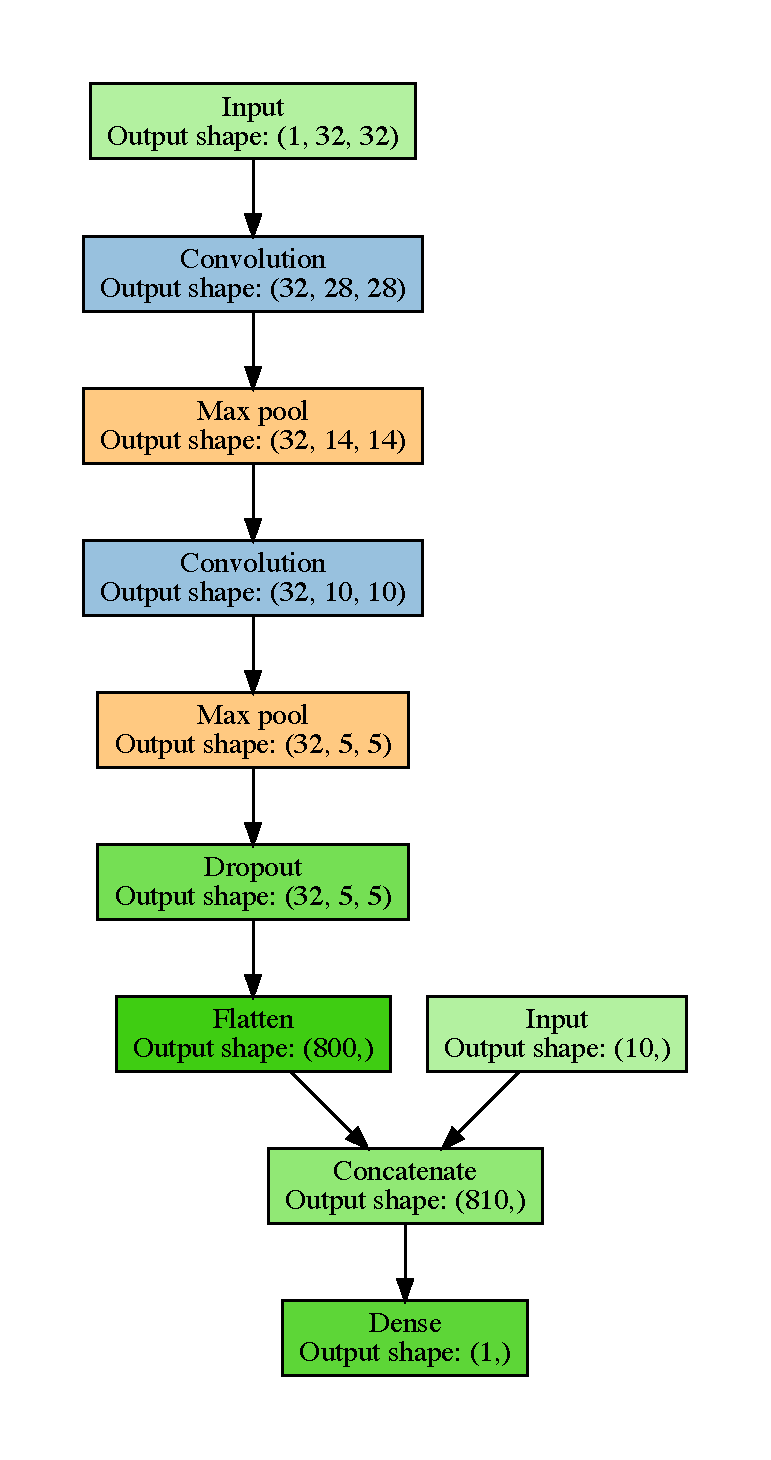
\includegraphics[width=\linewidth]{images/cnn_model_graph}
        \caption{Architecture of our CNN. The concatenate layer flattens the
          output of the previous layer and adds the 10 features derived from
          the candidate host in SWIRE, i.e. the flux ratios, stellarity
          indices, and distance. The dropout layer randomly sets $25\%$ of its
          inputs to zero during training to prevent overfitting. Diagram based
          on \url{ https://github.com/dnouri/nolearn}.}
        \label{fig:cnn}
      \end{figure}

      CNNs have recently produced good results on large image-based datasets
      in astronomy \citep[e.g.][; Lukic et al. in prep]{dieleman15cnn}. We
      employ only a simple CNN model in this paper as a proof of concept that
      CNNs may be used for class probability prediction on radio images. The
      model architecture we use is shown in \autoref{fig:cnn}.

    \subsection{Random Forests}
    \label{sec:random-forests}

      Random forests are an ensemble of decision
      trees~\citep{breiman01random-forest}. It considers multiple subsamples
      of the training set, where each bootstrap subsample is sampled with
      replacement from the training set. For each subsample a decision tree
      classifier is constructed by repeatedly making axis-parallel splits
      based on individual features. In a random forest the split decision is
      taken based on a random subset of features. To classify a new data
      point, the random forest takes the weighted average of all
      classifications produced by each decision tree.

%%%%%%%%%%%%%%%%%%%% REFERENCES %%%%%%%%%%%%%%%%%%
\bibliographystyle{mnras}
\bibliography{rgz-cdfs-ms}


% Don't change these lines
\bsp	% typesetting comment
\label{lastpage}
\end{document}
